\section{光的反射}\label{sec:1-2}

光射到物体表面上的时候,有一部分光会被物体表面反射回去。
这种现象叫做\textbf{光的反射}。 这一节我们就来研究光的反射。

光射到任何物体的表面,都会发生反射。我们选择对光反射能力强的平面镜来研究光的反射。
一束光照射到镜面被反射回去,可以看出,反射光仍然沿直线传播。
那么,反射光线的方向是由什么决定的呢?它跟照到镜面的入射光线有什么关系呢?
我们用如图 \ref{fig:1-4} 所示的装置来研究这个问题。

\begin{figure}[htbp]
    \centering
    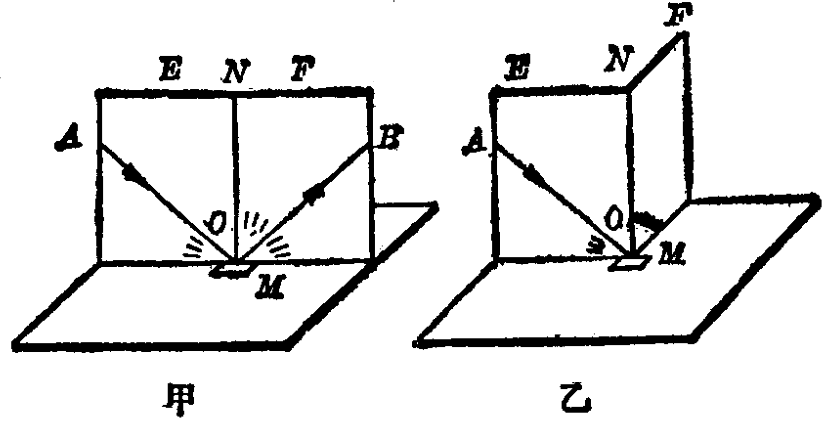
\includegraphics[width=0.7\textwidth]{../pic/czwl2-ch1-4}
    \caption{光的反射}\label{fig:1-4}
\end{figure}

$M$ 是平面镜,镶在一块木板上,在木板上立一块带有半圆刻度的白色屏,用来显示光束传播的路径。
这个屏是由两块长方形硬纸板 $E$、$F$ 粘连起来的,它们可以绕着接缝 $ON$ 向前折或者向后折。
把 $E$ 竖直地固定在木板上,然后让一束光沿 $E$ 上的 $AO$ 射到平面镜上的 $O$ 点。
转动 $F$,当它跟 $E$ 在同一平面时,就会在 $F$ 上看到有光束沿 $OB$ 射出(图 \ref{fig:1-4} 甲);
当 $F$ 在别的拉置时,就看不到反射光了(图 \ref{fig:1-4} 乙)。

我们把通过入射点 $O$ 垂直于镜面的直线 $ON$ 叫做\textbf{法线}。
从上面的实验可以看出,反射光线跟入射光线和法线在同一平面上。

在上面的实验里,还可以从屏上的圆形刻度盘上观察入射光线和反射光线的方向。
我们把入射光线 $AO$ 跟法线 $ON$ 的夹角 $\angle AON$ 叫做\textbf{入射角},
     反射光线 $OB$ 跟法线 $ON$ 的夹角 $\angle BON$ 叫做\textbf{反射角}。
让入射光线 $AO$ 沿不同的方向射入,观察反射光线 $OB$ 的方向,可以看出反射角总是等于入射角。

这样,我们就得到了光的\textbf{反射定律:
反射光线跟入射光线和法线在同一平面上,
反射光线和入射光线分居在法线的两侧;
反射角等于入射角}。

\begin{figure}[htbp]
    \centering
    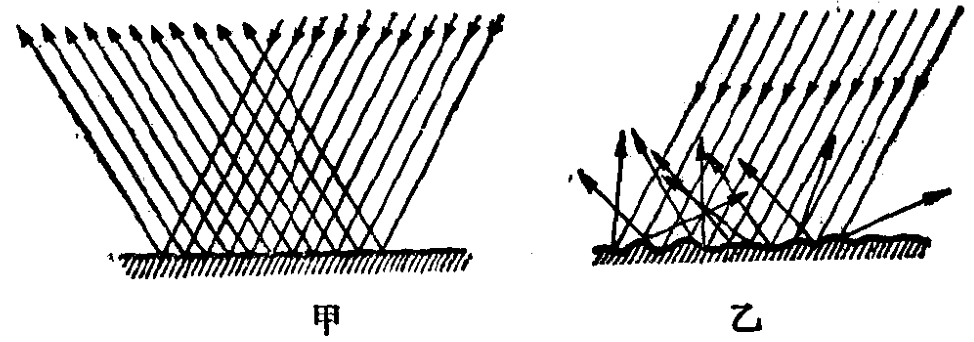
\includegraphics[width=0.7\textwidth]{../pic/czwl2-ch1-5}
    \caption{镜面反射(甲) 和漫反射(乙)}\label{fig:1-5}
\end{figure}

光射到任何表面上都会发生反射,但是从生活经验知道,不同的表面对光的反射是不一样的。
平滑的表面,例如镜面、抛光的金属面、平静的水面等;能使平行的入射光线沿着同一方向反射出去,
即反射光线也是平行的(图 \ref{fig:1-5} 甲)。
因此在这一方向上的反射光就强,而在其他方向上没有反射光。这种反射叫做\textbf{镜面反射}。
如果表面粗糙不平, 即使入射光线是平行的,反射后的光线也不平行,而是射向各个方向(图 \ref{fig:1-5} 乙)。
这种反射叫做\textbf{漫反射}。
必须注意,发生漫反射的时候,每一条光线还是遵守反射定律的。

一般物体的表面都是粗糙不平的。纸张、桌面、布等看起来是平的,可是仔细观察就知道都有些微小的凸凹不平。
光射到这些物体表面上的时候,就发生漫反射。
我们能从不同的方向看到这些本身不发光的物体,就是因为它们的表面能把射来的光向各个方向反射的缘故。

